\documentclass[11pt]{article}
\usepackage{graphicx}
\usepackage[nottoc,numbib]{tocbibind}
\usepackage[a4paper, total={6in, 8in}]{geometry}
\usepackage{titling}
\usepackage{fancyhdr}
\pagestyle{fancy}
\fancyhead{}
\renewcommand{\headrulewidth}{0pt}
\fancyfoot[LE,RO]{Y1481702}
\newcommand{\myparagraph}[1]{\paragraph{#1}\mbox{}\\}

\title{Software Testing}
\author{Y1481702}
\date{\today}
\setlength\parindent{0pt}
 
\begin{document}
\begin{titlepage}
\clearpage\maketitle
\thispagestyle{empty}
\tableofcontents
\end{titlepage}

%Your report must not exceed 10 sides of A4, minimum of 11pt font
%minimum 120% line spacing
%o: correct, see https://tex.stackexchange.com/questions/348678/how-to-set-document-line-spacing-in-pt-format
%minimum 2cm margins on all sides

%does not include covering page, table of contents or reference list

%EXAM NUMBER SHOULD BE WRITTEN ON THE FRONT PAGE AND ALL SUBSEQUENT PAGES
%APPROX ONE PAGE PER 10 MARKS:


%GENERAL ADVICE:
	%You won’t receive marks for testing that the marker merely thinks you probably did — marks will only be awarded for tests that are described explicitly and precisely.
	%Yes, it is a little unrealistic that you are only allowed 10 pages and 8 tests, and that your possible coverage and comprehensiveness are limited by that. However, in the real world there are always resource limits — the ones you have here are merely artificial ones.
	%Do not repeat anything that does not vary. For example, do not repeat the same boilerplate text in every test case description — if something is true for all test cases, say this once at the start of the section.
	%Similarly, use blanket statements to make points that are true of multiple (but not all) tests case (e.g. “Test cases 1–5 assume that...”)
	%Appendices containing full JUnit code or detailed test output etc are not required and will not be read.
	%In general, do not waste space on spurious information. Think about what the notional target reader needs to know in order to use your document, and include only that. At best, other information will waste some of the limited pages available to you.
	%If you reference an external document (such as the documentation or website for the software you are testing), be sure to cite it appropriately, just as in any other submitted work.

\section{Test Plan}% 25 Marks (2.5 pages)
%A test plan
%It should detain the methods used to build the test cases and the software tools used to achieve these
\subsection{Introduction}
%o: What is JAVA MASON?
Java MASON is an agent-based..

%o: From a testing point of view MASON is a form of OPEN SOURCE SHRINKWRAP
	%may be used in the wild by many people
	%what other ramifications does this have
The software fits into the category of shrinkwrap meaning it may be used by many people in a variety of ways.

%usage statistics can provide with an estimate of how well it needs to work
%biological simulations- high profile studies have based hypotheses on this framework
In particular, 

The software is freely-available and open-source, which is a special case of shrinkwrap software.
%As open source software is often developed without anyone being paid,
	%only "fun" things are done
	%i.e. NOT TESTING
While some form of automated testing may have been conducted, it cannot be taken for granted as this has not been distributed with the source code, either on the MASON website, or its GitHub repository.

\subsubsection{Tools}
The IntelliJ IDE was used to explore the code and develop automated tests.
JUnit has been used to create automated unit tests for the software.
UI tests?
\\

Git version control has been used to manage the code for the JUnit tests. For a long term project, this would mean that automated tests could be updated alongside any code changes.

\subsection{Test Coverage}
%Clearly define what constitutes "the software under test" and list the features that you will test and not test
As stated in the project brief, the testing only needs to cover the \texttt{sim.engine}, \texttt{sim.field} and \texttt{sim.field.grid} packages, but not their subpackages.
\begin{itemize}
\item \texttt{sim.engine} is responsible for the core simulation management, including the agent scheduling.
\item \texttt{sim.field} provides abstract classes for the representations of space in MASON simulation models, with subpackages managing specific instances of these.
\item \texttt{sim.field.grid} provides various 2D and 3D grid representations of simulation space.
\end{itemize}

%Explain how you have determined the expected behaviour of the software (in the absense of an exhaustive and explicit requirements specification)
The expected behaviour of the software has been determined using the extensive Java MASON documentation\cite{mason_doc}, first-party example implemtations as well as a number of open-source examples\cite{ppsim}.
%usage by a private biological research institute
%users will be research scientists with BASIC Java training
The system behaviour has been tested against the inferred requirements of the client, a private biological research institute.
%Explain the overall strategy you used for creating test cases, and for selecting the specific test cases that you present in section B
\\

In order to design appropriate test cases an understanding of all levels of the system was needed.
%how do we know how a general user works?
%examples of real-world usage (PPSim), vs mason tutorials
IntelliJ's Diagram feature helped to show how different components of the system are connected.
Code coverage has provided a good understanding of which parts of the [code] are regularly used while running the software.
Other metrics, such as how often different source files have been changed provide an insight into which files are most subject to change.

%Define acceptability criteria for the software - what (testable) properties does it need to have in order for it to be acceptable quality for its intended purpose?
%o: These will help define the goals of our testing:
	%find the maximum number of bugs?
	%know whether we have undiscovered bugs?
	%comply with regulator-set demands

	%have a compelling defence in a courtcase (self-driving cars, too soon?)
	%minimum time and cost?
		%obviously here we have a set TIME- open assessment for 10 credit module



\section{Test Case Specifications}% 30 Marks (3 pages)
%Test case specifications for 8 fully specified test cases. The test cases must be complementary: they must make different assumptions and test different specific features of the library.
	%At minimum, each test case should describe the stimulus applied to the software (which might be a sequence of API calls, a sequence of user actions that are taken, or something else) and the expected
		%i.e. correct behaviour
		%N.B. for some tests it may be appropriate to define constraints (e.g. "no files will be changed") instead of/as well as positive statements of behaviour (e.g. "the user will be returned to the main menu screen").
		%Where the reason why the expected/correct behaviour is indeed expected and correct is not obvious to a capable programmer where some domain knowledge, explain briefly why it is so
	%Each test case should also state the purpose of the test within the test set. A good way to do this may be to state the question that the test case asks about the software. If we cannot understand what the purpose of a given test case is, we cannot give you much credit for it.
	%“One test case” should test one thing – one feature, one unusual input, or one user task. For example, if you have a function that takes an integer as an input, testing it with Min/Max/+1/0/-1 should be five test cases. One can note that those are, however, five very low-level (unit test) test cases, which are unlikely to give you the most testing power in a fixed number of tests, and hence unlikely to give you maximum marks.
	%You should aim to provide a diverse range of test cases, and also to provide your best test cases (including any that find interesting bugs). There is an inevitable tension between these two objectives, which you will have to decide how to resolve.
	%For full marks in this section, tests should be conducted at a range of testing levels, including unit, integration and system level. Hint: explicitly label each of your tests with what level it’s working at.
	%You may include short fragments of code within your test case specifications, but not larger ones. In particular, do not include whole JUnit tests. In essence, you need to provide enough information for a smart programmer to recreate your test code given some effort. e.g. if a test case involves a specific sequences of method calls, that sequence of method calls needs to be clear from the test case description.


%o: "Black box testing means that knowledge of the internals of the product doesn't play a significant part in your testing."\cite{lessons_book}
%o: "To do black box testing well, learn about the user, their expectations and needs, the technology and configurations the software will run on, the other software that this software will interact with, the date the software must manage, the development process, and so on. The advantage of black box testing is that you probably think differently than the programmer, and, thus are likely to anticipate risks that the programmer missed."
\subsection{Test 1}
\subsection{Test 2}
\subsection{Test 3}
\subsection{Test 4}
\subsection{Test 5}
\subsection{Test 6}
\subsection{Test 7}
\subsection{Test 8}

\section{Test Results}% 15 marks (1.5 pages)
%The test results for each of the tests that were specified in item B.
	%Here, you should document the results that occurred when the test cases are run. You should provide explicit indication of whether each test passed or failed, and in the latter case state what happened instead.

%o: screenshots may be useful, but add them in appendix?
\subsection{Test 1}
\subsection{Test 2}
\subsection{Test 3}
\subsection{Test 4}
\subsection{Test 5}
\subsection{Test 6}
\subsection{Test 7}
\subsection{Test 8}

\section{Test Summary Report}% 30 marks (3 pages)
%A test summary report that will contain at least:
	%a summary of the testing that you performed
	%a summary of the results you observed, including a classification of the faults found (by an appropriate classification scheme of your choosing)
	%an overall evaluation of the thoroughness and quality of the testing you have performed
		%o: code coverage results for unit testing?
		%This should be in terms of what might be possible given substantial resources, not in terms of what is possible in a project with this time allocation and maximum report length.
		%Describe the branch coverage and condition coverage, or the mutation score according to a reasonable mutation testing approach, that your tests achieved of the Java code (not of any other artefact). Briefly explain how you did it; make sure you state what tools you used and (where applicable) what mutation operators you used.
	%an overall evaluation of the software tested (in terms of its freedom from faults)
		%o: obviously due to time and limitations on the number of test cases, this is a limited assessment
		%o: but OVERALL..?

	

%Throughout, the summary report should only refer to the test cases that were specified in (B), not any other testing you may have performed.

\newpage
\raggedright
\bibliography{Report}{}
\bibliographystyle{ieeetran}
\newpage
\section{Appendix}
\begin{figure}[htp]
\centering
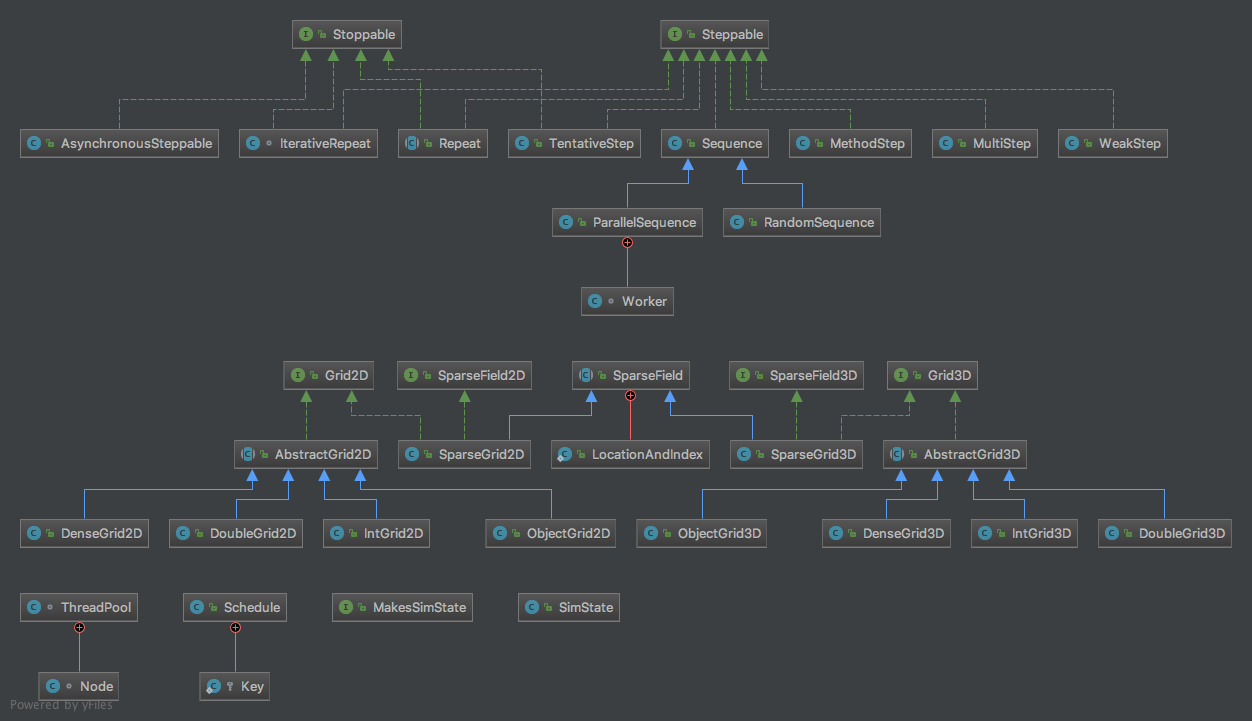
\includegraphics[width=\textwidth]{Appendix/UML}
\caption{Reverse Engineered UML diagram of Class Hierarchy}
\label{fig:uml}
\end{figure}

\end{document}